
\documentclass{amsproc}
 
\usepackage{graphicx}
\usepackage{amsmath}

\newtheorem{theorem}{Theorem}[section]
\newtheorem{lemma}[theorem]{Lemma}

\theoremstyle{definition}
\newtheorem{definition}[theorem]{Definition}
\newtheorem{example}[theorem]{Example}
\newtheorem{xca}[theorem]{Exercise}

\theoremstyle{remark}
\newtheorem{remark}[theorem]{Remark}

\numberwithin{equation}{section}

%    Absolute value notation
\newcommand{\abs}[1]{\lvert#1\rvert}

%    Blank box placeholder for figures (to avoid requiring any
%    particular graphics capabilities for printing this document).
\newcommand{\blankbox}[2]{%
  \parbox{\columnwidth}{\centering
%    Set fboxsep to 0 so that the actual size of the box will match the
%    given measurements more closely.
    \setlength{\fboxsep}{0pt}%
    \fbox{\raisebox{0pt}[#2]{\hspace{#1}}}%
  }%
}

\begin{document}

\title{Incorporating stochasticity in simple models of disease  spread}

%    Information for first author
\author{Jonathan Dushoff}
%    Address of record for the research reported here
\address{Department of Biology, McMaster University, Hamilton, Ontario L8S-4K1}
\email{dushoff@mcmaster.ca}
%    \thanks will become a 1st page footnote.
\thanks{This work was supported by the National Science and Engineering Research Council of Canada}


\maketitle

\newcommand{\Nasell}{N\aa sell}
\newcommand{\et}{\emph{et~al.}}
\newcommand{\etc}{etc.\ }
\newcommand{\eg}{\emph{e.g.\ }}
\newcommand{\ie}{\emph{i.e.\ }}
\newcommand{\dfe}{disease-free equilibrium}
\newcommand{\cf}{\emph{cf.\ }}
\newcommand{\Rx}{\mbox{$\cal R$}}
% \newcommand{\ct}[1]{((#1))}
\newcommand{\ct}[1]{\cite{#1}}
% \newcommand{\Rs}{\mbox{$\cal R^*$}}
\newcommand{\Ro}{\ensuremath{R_0}}
\newcommand{\ro}{\mbox{$\rho$}}
\newcommand{\ds}{\displaystyle}
\newcommand{\fref}[1]{Figure \ref{#1.fig}}
\newcommand{\figlab}[1]{\label{#1.fig}}
\newcommand{\tref}[1]{Table \ref{#1.tab}}
\newcommand{\tlab}[1]{\label{#1.tab}}
\newcommand{\eref}[1]{(\ref{#1.eq})}
\newcommand{\eqlab}[1]{\label{#1.eq}}
\newcommand{\aster}{$\mbox{}^*$}
\newcommand{\up}[1]{$\mbox{}^#1$}
\newcommand{\blk}{\obeylines\setlength{\parskip}{0ex}\medskip}

\newlength{\figwidth}\setlength{\figwidth}{0.8\hsize}
% \newcommand{\includegraphics}[1]{{\bf (Figure #1 here)}}

\maketitle

As we have seen in earlier chapters, simple models of infectious diseases in homogeneous populations have produced many important insights.  The most basic of these is the basic reproductive number $R_0$, and its corollaries: the population (or `herd') immunity threshold; and the qualitative shape of the relationship between $R_0$, disease parameters and endemic levels of disease.  Another key idea is the cyclic tendency of epidemic outbreaks, and the natural tendency of these oscillations to be damped.

Although such models have produced important insights, it is important to bear in mind that they are simple (albeit useful) approximations to a much more complex reality.  Thus, it is also useful to consider what the key simplifications of these models are, and ways in which their predictions might change when various complications are added.  Several such complications may be loosely grouped under the classification of ``heterogeneities": populations in the simple models we have learned about are fundamentally homogeneous.

Examples of heterogeneities not accounted for in simple models include ``parametric heterogeneity", ``geographic heterogeneity" and ``demographic heterogeneity."  Parametric heterogeneity refers to individual differences in transmission parameters for a particular disease; for example, differences among individuals in contact rate, susceptibility to infection, or tendency to transmit disease.  Starting with the work of Hethcote and Yorke \ct{HethYork84}, parametric heterogeneity has been shown to pervasively affect the relationship between risk factors and disease -- on the whole, tending to make disease levels less sensitive to increases and decreases in risk \ct{Dush99}. 

Geographic heterogeneity refers to the geometry of interaction networks between people; people do not mix homogeneously, but instead mixing is structured by spatial location, social networks, and other factors.  The effects of geographic heterogeneity on disease spread is an active research area, which is further divided (loosely) into spatial models (see, e.g., \ct{Rile07}) and network models (e.g.,\ct{BansGren07}).  This chapter will focus on demographic heterogeneity.  A good source for further reading on this subject is \ct{AlleBook}.

\section{Modeling demographic heterogeneity}

Demographic heterogeneity refers to the heterogeneity introduced simply by treating individuals as individuals.
To see what this means, we first ask what happens in a classic, ODE model of disease, if we introduce a single infectious individual to a susceptible population.
If $\Ro>1$, after a short period of time, we deterministically find something like 1.1 infectious individuals, whereas if $Ro<1$, after a short period of time we have 0.9 infectious individuals.

In reality, of course, a single infectious individual does not increase smoothly to 1.1 infectious individuals.  
Instead, the system will take a discrete jump, either to 2 infectious individuals or to 0.
We cannot reasonably expect to specify a model of disease transmission in enough detail that we can predict exactly when the next event of each type will occur.
Instead, simple models that include discrete events are fundamentally stochastic; even in theory we don't know when the next event will occur, nor even what it will be.

Thus, if we treat individuals as individuals, we necessarily introduce ``demographic" stochasticity, defined as stochasticity caused by the existence of individual people and discrete events.   Stochasticity may also operate at a larger scale; we refer to events outside our model that affect more than one person at a time as ``environmental" stochasticity.  In a model of disease spread in human populations, sources of environmental stochasticity would include weather and economic change, for example.

This is illustrated in \fref{onestoch}.  The deterministic trajectory starts from a single introduction and increases smoothly to around 2.5 infectious individuals.  In contrast, the stochastic trajectories move in discrete, unpredictable jumps.  Some of them randomly increase to as high as 8 or 9 infectious individuals, while in one case, the disease goes extinct before the end of the week.

\begin{figure}
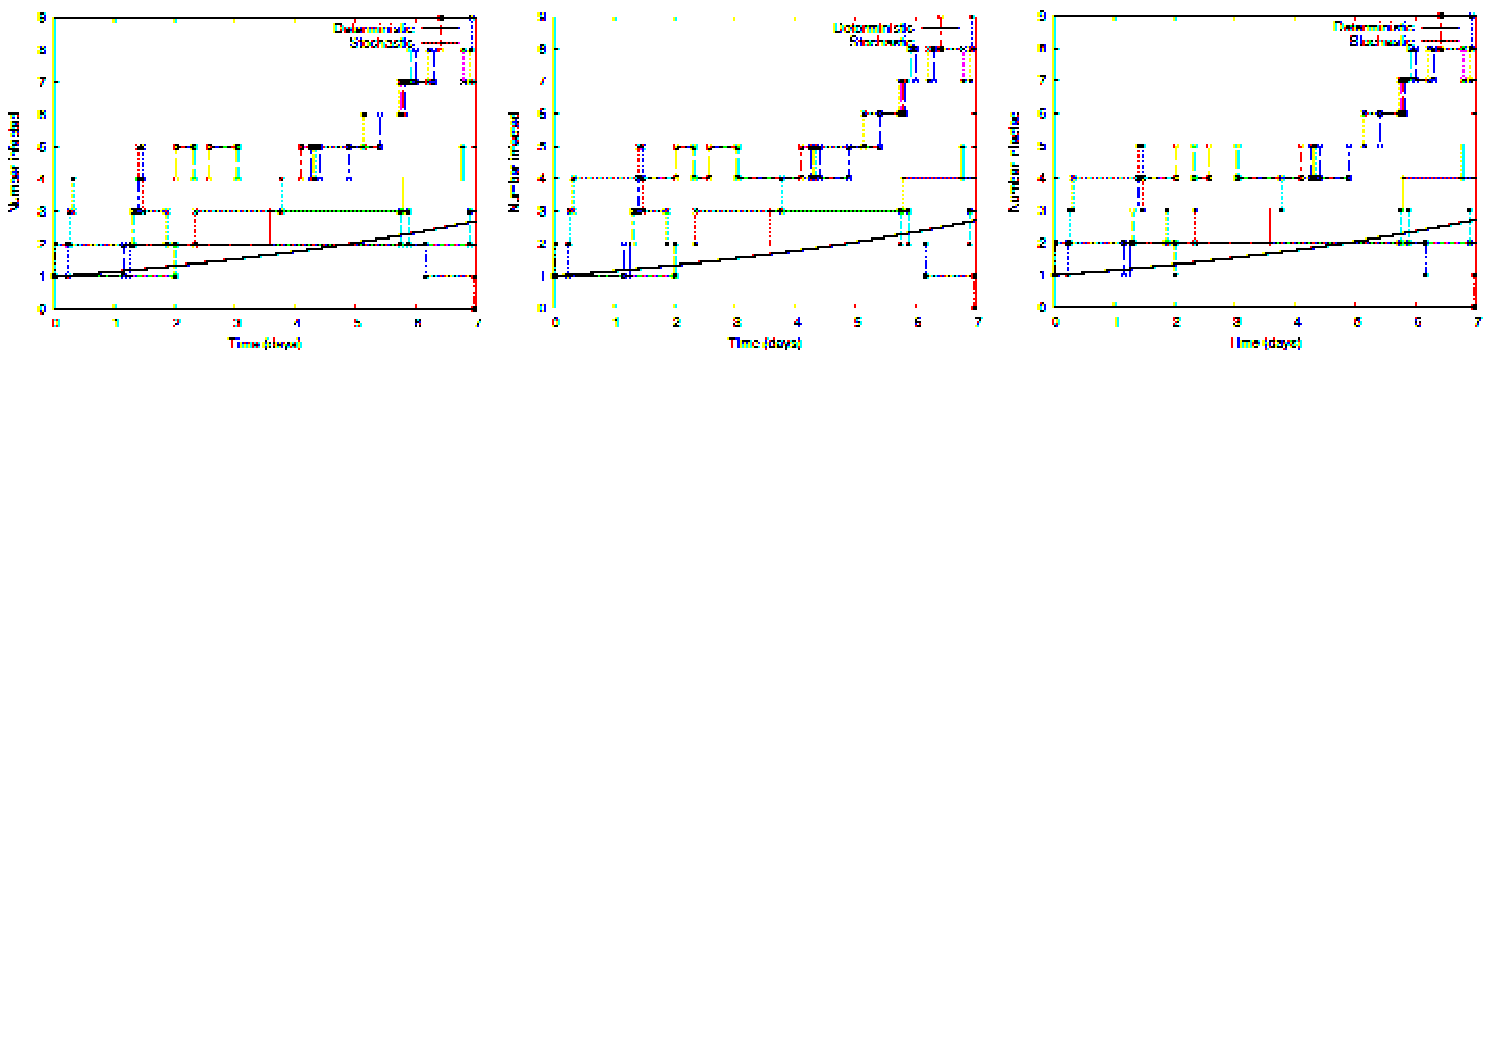
\includegraphics[width=\figwidth]{inputs/stochcomp.pdf}
\caption[Demographic spread]{
%
	The deterministic trajectory from a simple SIR model \eref{ode} is compared with several trajectories from an analogous stochastic model (\tref{rates}).  Parameters are $\Ro=2$, $\rho=0.01$.  The disease generation time is 7 days.
%
}
\figlab{onestoch}
\end{figure}

\section{Describing a demographic model}

Interestingly, there is a natural way of translating a simple ODE model directly into an analogous discrete-individual model.  
This being so, it is useful to investigate how the behavior and predictions SIR models are changed by the inclusion of this realistic effect.

To create a discrete-events model, we describe our system in terms of the {\em probability rates} of events happening. 
If the rate of event $E$ is $r_E(t)$, the probability of the event occurring in the time interval $(t, t+dt)$ is $r_E(t) dt$. 
If the system is {\em Markovian}, $r_E(t)$ depends only on the state of the system at time $t$. 
If the system is {\em non-Markovian} $r_E(t)$ can depend (for example) on how long the system has been in a particular state.

The Markovian assumption allows us to specify the state of our system with a much smaller amount of information, but it can have unwanted consequences.  
In particular, assuming that residence in a particular state is independent of history is equivalent to assuming that the residence time in that state is exponentially distributed.
This assumption is often strikingly unrealistic -- for example, in a human population with exponentially distributed lifetimes and a mean lifetime of 70 years, 5\% of people will live to be over 200 years old!  
Thus, we must question the extent to which our results depend on this extremely convenient, but unrealistic, assumption.

\begin{figure}

{
	\setlength{\unitlength}{1.0cm}

	\begin{picture}(12,4)

	\put(0.5,1){\framebox(2,2){S}}
	\put(4.5,1){\framebox(2,2){I}}
	\put(8.5,1){\framebox(2,2){R}}

	\put(2.5,2){\vector(1,0){2}}
	\put(6.5,2){\vector(1,0){2}}
	% \put(9,1.8){\vector(-1,0){2}}

	\put(1.5,1){\vector(0,-1){1}}
	\put(5.5,1){\vector(0,-1){1}}
	\put(9.5,1){\vector(0,-1){1}}

	\put(1.5,4){\vector(0,-1){1}}

	\put(0.9,3.5){$\rho N$}
	\put(1.6,0.5){$\rho$}
	\put(5.6,0.5){$\rho$}
	\put(09.6,0.5){$\rho$}

	\put(3.2,1.7){$R_0 I/N$}
	\put(7.4,1.7){$1-\rho$}

	\end{picture}

}

\caption[Box model]{
%
	A diagrammatic model of the spread of an infectious disease.  
	Individuals may be {\bf S}usceptible, {\bf I}nfectious, or {\bf R}esistant.
	Susceptible individuals move to the infectious category at a rate proportional to the number of infectious individuals present.  
	Births, deaths and recovery from disease into the Resistant class occur at constant rates.
%
}
\figlab{sir}
\end{figure}

\fref{sir} shows a diagram of an infectious disease model.  
By counting time in units of infectious disease generations, and populations as fractions of the total population, we can reduce this simple, but by no means trivial, model to only two parameters, the basic reproductive number \Ro; and \ro, which represents the ratio between the two fundamental time scales of the model: the average infectious period, and the average duration of immunity following infection.
\begin{equation}
	\begin{split}
		\dot x &= \rho(1-x) - R_0 xy \\
		\dot y &= R_0 xy - y
	\end{split}
	\eqlab{ode}
\end{equation}
Here, $x$; $y$ refer to the proportion of the population infectious; susceptible.  
Since we assume a constant population, we are free to drop the equation for the proportion in the removed class.  The dots refer to derivatives with respect to time.

\begin{table}
\begin{center}\begin{tabular}{llll}
   {\bf Event} & {\bf transition} &{\bf rate} &{\bf Effect $(S,I)$}\\
   \hline
   Infection &$S \to I$  &$R_0 SI/N$ & $(-1,1)$\\
   Recovery & $I \to R$ & $(1-\rho)I$ & $(0,-1)$\\
   Rebirth &  $R \to S$ & $\rho (N-S-I)$ & $(1,0)$\\
   Rebirth & $I \to S$ & $\rho I$ & $(1,-1)$
\end{tabular}\end{center}
\caption[Rates table]{
%
	We specify a demographic model by describing the events that can occur; the way that the rates of these events depend on the state of the system; and the effect of these events on the variables that describe the state of our system.
%
}
\tlab{rates}
\end{table}

\tref{rates} shows how we re-cast the model in \fref{sir} as a demographic model, reflecting a population composed of discrete individuals.
Each arrow represents an event that can occur stochastically, affecting a discrete individual, with a probabilistic rate that corresponds to the deterministic rate in \eref{ode}.  
We will discuss below how this stochastic model of the disease system in \fref{sir} can be either simulated, or analyzed.  Note that the model given by \tref{rates} cannot be parameterized as simply as the one in \eref{ode}; if individuals are discrete, the population size $N$ will fundamentally affect the behavior of the model.

The demographic model is an exact analogue of the deterministic one, both conceptually, and in the technical sense that as the population size $N\to\infty$ in the demographic model, its behavior converges to that of the deterministic model.  
Although we can convert a demographic model to a deterministic model simply by allowing the population size to go to infinity, translating a deterministic model to a demographic one requires us to make choices about how to group the terms in our model into events.  For example, the two transmission terms in our simple model -- the contribution of $-\Ro xy$ to $\dot x$, and the contribution of $\Ro xy$ to $\dot y$ -- clearly refer to the same event: an individual moves from the susceptible class to the infectious class.  Less clear is the interpretation of birth and death terms.  We could choose to interpret the model \eref{ode} as having independent birth and death events -- and thus, stochastic fluctuations in population size -- or we can choose (as we do in \tref{rates}) to link these birth and death events, and keep the population constant.

Having described a model that takes demographic stochasticity into account, we can now begin to ask questions about the expected effects of demographic stochasticity on disease dynamics. 
In particular, we can now ask questions about the {\em probability} of establishment or persistence of diseases with $\Ro>1$.  We can also ask how we expect demographic stochasticity to affect temporal dynamics of diseases, and how much variability we expect to see due to demographic stochasticity.

\section{The behavior of a stochastic model}

We have experience in interpreting the behavior of deterministic models.  
Given parameters, and a starting point, we examine the predicted trajectory of the model.  
We also have techniques for combining information from different starting points into phase planes, and information using different parameter sets into bifurcation diagrams.

For stochastic models, we must re-evaluate what we mean by the ``behavior'' of a system.  
Given parameters, and a starting point, we do not know what the trajectory of the model will be.  
We can attempt to simulate a random sample of what the model might do.  Such an example of a single trajectory is called a {\em realization}. 
We can attempt to characterize the universe of all possible such realizations; this is called the {\em ensemble}; we can imagine the ensemble as an infinity of realizations running simultaneously.
Less ambitious than attempting to characterize the whole ensemble, we could ask about the probability distribution that describes what state we expect the population to be in at any given time; this is called the {\em ensemble distribution}. 

We have a variety of techniques available to interpret a stochastic dynamical system.  
1) Most straightforwardly, we can simulate one or many realizations.   
2) We can simulate the entire ensemble distribution; this technique is restricted to systems with relatively small population size, since such  simulations require that we keep track of one state variable for each possible state of the system. 
3) We can solve the ensemble distribution dynamics exactly; this is possible only in special cases, but these solutions can be enlightening.
4) We can construct analytic {\em approximations} to the ensemble distribution.

\subsection{Simulating individual realizations}

Continuous-time models with discrete events can be simulated in a straightforward manner, outlined below \tref{gillespie}.  This method has been known for at least half a century, and is attributed to Kendall by \ct{Bart61}.  It was explicated in detail by Gillespie \ct{Gill76}, and is often referred to as the Gillespie method.
Briefly, given that rates are known, we can infer the distribution of the waiting time to the next event, as well as the probability that the next event is of any particular type.  By iterating, we can simulate a stochastic realization.

\begin{table}

{\bf Simulating a realization}

\begin{itemize}

	\item Given a state of the system: 

	\begin{itemize}

		\item List possible events, and associated rates. 

		\item Randomly select the time and nature of the next event:

		\begin{itemize}

			\item Calculate the total rate $r_T$

			\item the next event will happen after an exponential waiting
			time with mean 1/$r_T.$ 

			\item The probability of event $E$ is $r_E/r_T$. 

		\end{itemize}

		\item Change the system state appropriately. 

	\end{itemize}

	\item Repeat forever. 

	\item Or until disease is extinct. 

	\item Or until you are tired 

\end{itemize}
\caption[Gillespie]{
%
	Steps in simulating a demographic model.
%
}
\tlab{gillespie}
\end{table}

\begin{figure}
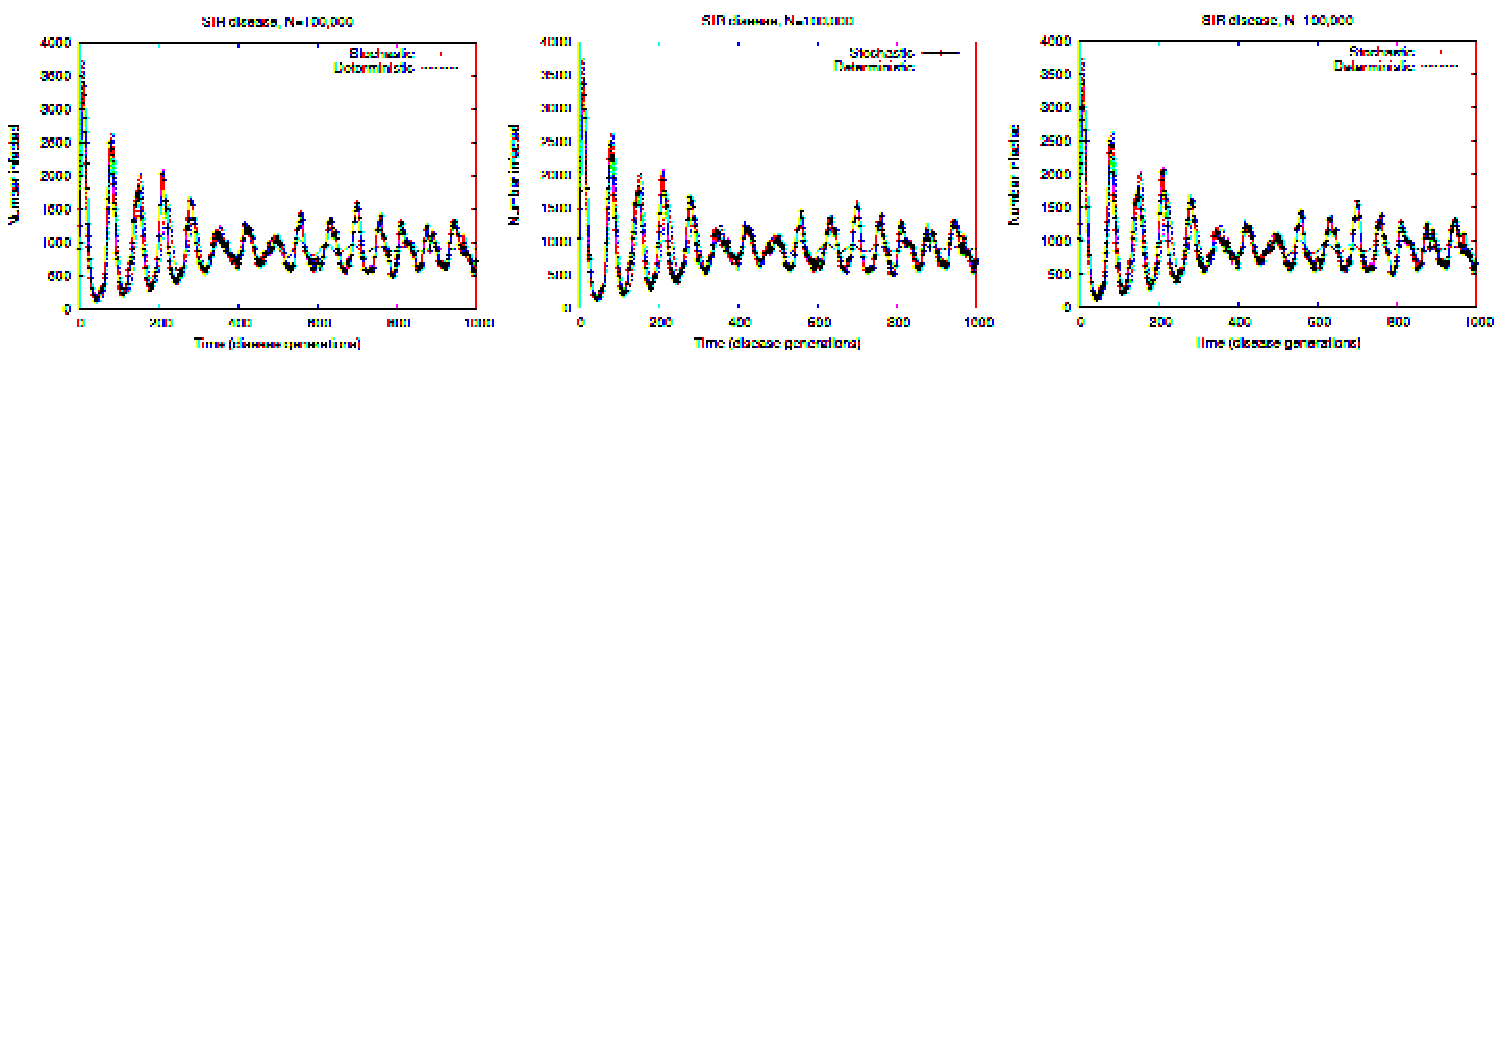
\includegraphics[width=\figwidth]{inputs/dscomp.pdf}
\caption[Demographic spread]{
%
	The deterministic trajectory from a simple SIR model \eref{ode} is compared with a typical stochastic trajectory from an analogous stochastic model (\tref{rates}).  Parameters are $\Ro=10$, $\rho=0.001$, $N=1,000,000$.  The system was started relatively close to the endemic equilibrium (with 120,000 susceptibles) to avoid too violent a first epidemic.
%
}
\figlab{comp}
\end{figure}

\subsection{Simulating the ensemble distribution}

We model the ensemble distribution by creating one conceptual `box' for each possible state of the system, and asking what is the probability that the system is in each box. 
Conceptually, this approach is surprisingly simple; the catch is that there may be a lot of boxes -- in fact, one for each possible state of the system.
In an SIS model with fixed population size, we might have effectively only one state parameter in the deterministic model. 
In this case, the number probabilities to model in the ensemble distribution is of order $N$, the population size.
In an SIR model, we need at least two deterministic state variables, so the number of discrete state probabilities will be of order $N^2$ -- or $N^3$ if we allow population size to vary, or take disease latency into account \ldots.  

Since the human global population is on the order of $10^{10}$ individuals, with major cities having $>10^5$ individuals, this approach quickly becomes prohibitive.  Nonetheless, we may gain valuable information from our investigations of simpler cases.

Although often difficult in practice, simulating an ensemble distribution is conceptually straightforward.  
Given our event rates, we can determine the rate of {\em direct} transit between any to states $S$ and $S'$.  
This rate will of course be zero in many cases.
It is then straightforward to write equations for how the probabilities of being in a given state $p(S)$ change through time:
\begin{equation}
	\dot p_S =
	\sum_{S'}{p_{S'} r_{S'\to S}} -  p_S \sum_{S'}{r_{S\to S'}}  
	\eqlab{distribution}
\end{equation}

\section{Analytic approaches}

In addition to simulating equations of the form \eref{distribution}, we may also seek analytic understanding.
Rather remarkably, in some cases equations of this form can be solved exactly for interesting biological systems.
Although these examples are necessarily very limited, such exact solutions can be very illuminating.

We might also seek approximate analytic solutions to increase our understanding.   
These two approaches are related, since an exact solution to a simplified problem may in some cases serve as an approximate solution to the original problem.  
In addition to such simplifications, analytic approximation techniques that can be applied include moment approximations and diffusion approximations.

Two of the most useful tools for understanding deterministic disease models are based on linearizations.  
We linearize around the disease-free equilibrium to investigate what factors control whether the disease can invade and persist. 
We linearize around the endemic equilibrium to investigate the system's tendency to cycle, and the characteristic period and damping time of cycles.  
Both of these methods have analogues in demographic models (see below): the linear birth-death model is based on linearizing about the disease-free equilibrium, and diffusion approximations are based on linearizing about the endemic equilibrium.

\subsection{The fate of an introduced disease}

Consider for a moment the long-term fate of a realizations of our demographic system (\tref{rates}).  The total population always remains fixed, but on reflection we will see that {\em eventually} the disease will always go extinct: however large $N$, and however low the (average) probability of recovery before the next infection, in infinite time, we will always eventually throw $H$ tails in a row, so to speak.  

From a biological point of view, this fact may not seem very interesting, since the expected time to extinction of disease in our model will often dwarf the expected lifetime of the universe.  Mathematically speaking, however, it poses serious obstacles.  Investigating equilibria is a vitally useful mathematical technique, but the only real equilibrium of this system is the disease-free equilibrium.  Below, we will see how this concept is addressed with the concept of the quasi-equilibrium.

Beyond the observation that the disease must go extinct eventually, it is useful to categorize qualitatively different {\em ways} in which it might go extinct.  Based on the behavior of our system, we can identify either three (if we are mathematicians) or four (if biologists) such routes to extinction:

\begin{description}

	\item [Fizzle] the disease fails to cause an epidemic.  We will make this concept precise below

	\item [Burnout] the disease causes an epidemic, which reduces the number of susceptibles below the threshold required, and goes extinct before the level of susceptibles recovers (after the first epidemic)

	\item [Fadeout] the disease causes several epidemics, and approaches ``quasi-equilibrium'' (see below) before going extinct.

	\item [Persistence] the disease fades out, but after a biologically unreasonable period of time.  
	There is no convenient {\em mathematical} distinction between fadeout and persistence, but biologically it may make sense to make an arbitray distinction.

\end{description}

\subsection{Equilibrium and quasi-equilibrium }

We define equilibrium in our demographic system as an ensemble distribution that does not change with time. 
As noted above, the only equilibrium of the system is then the disease-free equilibrium. 
As long as any populations not extinct, proportion extinct will increase.
In particular, there is no equilibrium corresponding to the endemic equilibrium of the deterministic system. 
This is deeply inconvenient, since we would like to study such an equilibrium, to characterize how the system behaves in the long term.

We address the problem by constructing a ``quasi-equilibrium''. 
Consider the ensemble distribution confined to the subset of states where nothing is extinct. 
This system can be described as a {\em fully connected} (you can get anywhere from anywhere else, {\em open} (you can leave the set) flow. 
Intuition tells us that such a system has a unique, real, negative dominant eigenvalue, associated with a positive eigenvector. 
Linear algebra tells us this as well \ct{BermPlem79}.  Thus, the system will converge to a stable {\em relative} distribution of probabilities of being in each non-extinct box -- this relative distribution is called the quasi-equilibrium.

The quasi-equilibrium is the asymptotic probability of being in each system state with disease {\em given that the disease has not gone extinct.} 
The eigenvalue $\lambda_q$ associated with the quasi-equilibrium distribution is the rate at which the probability of non-extinction decays (exponentially). 
The distribution of persistence times must be asymptotically exponential. 
The expected persistence time (looking forward) approaches $-1/\lambda_q$ as the system continues to persist.

The quasi-equilibrium perspective also gives us a useful tool for numerical investigations.  
Just as we modeled the ensemble distribution above \eref{distribution},  we can also model the {\em conditional} probability of being in a particular state given that extinction has not occured. 
Since these probabilities converge in general to positive values (the quasi-equilibrium distribution), this approach tends to be computationally more stable than directly simulating the ensemble distribution. 
Since we can also keep track of the cumulative extinction probability, the information we obtain is equivalent. 
Define the conditional probabilities $q_S = p_S/(1-p_N)$, where $N$ is a `null' state that we cannot escape from.  Then we use the quotient rule to write equations for the conditional probabilities:
\begin{equation}
	\dot q_S = \sum_{S'}{q_{S'} r_{S'\to S}}
	-  q_S \sum_{S'}{r_{S\to S'}}  
	- q_S r_{S\to N}
	+ q_S \sum_{S'} q_{S'} r_{S'\to N},
\end{equation}
where the sums now go only over the states where the disease is not extinct.

\subsection{Linear birth-death process} 

In deterministic systems, we study disease invasion by asking how the number of infectives behaves in the limit where we assume that virtually the whole population is susceptible.
This is (typically) equivalent to linearizing about the disease-free equilibrium.
We take an analogous approach with stochastic disease models.
This corresponds to holding the number of susceptibles fixed at $N$; we are then left with a demographic model whose state is determined by the number of infectious individuals $I$. 
This system has only two events: 
\begin{table}
\begin{center}\begin{tabular}{llll}
   {\bf Event} & {\bf transition} &{\bf rate} &{\bf Effect on $I$}\\
   \hline
   Infection &$S \to I$  &$R_0 I$ & $1$\\
   Recovery & $I \to R$ & $I$ & $-1$
\end{tabular}\end{center}
\caption[Rates table]{
%
	We specify a demographic model by describing the events that can occur; the way that the rates of these events depend on the state of the system; and the effect of these events on the variables that describe the state of our system.
%
}
\tlab{linrates}
\end{table}

Surprisingly, the probability of eventual extinction in this system is not one.  
Our argument that the system must go extinct eventually breaks down, because the expected number of infectious individuals goes to $\infty$ in time.  
Thus, we can ask what is the extinction probability in this model.

This can be solved in a straightforward, and rather illuminating, fashion.
Chains of infection are independent in this model: since the rate at which an infection spawns new infections never changes, infectious individuals have no effect on the number of cases that will be caused by another infectious individual. 
We can use this fact to solve directly for the probability of extinction when starting from $I$ infections, $E_I$. 

If we start with one infectious individual, the probability that the next event will be a recovery (and thus that the disease will go extinct immediately) is $1/(R_0+1)$.  Otherwise, the next event will be an infection, and we will have two infectious individuals.
Thus:
\begin{equation}
	E_1 = \frac{1+\Ro E_2}{1+\Ro}.
\end{equation}

But, if our two new infectious individuals have independent chains of infection, the probability that they will both eventually go extinct is the product of the independent probabilities that each will go extinct: $E_2 = {E_1}^2$.  Thus, we have a quadratic equation for $E_1$:
\begin{equation}
	E_1 = \frac{1+\Ro {E_1}^2}{1+\Ro}.
\end{equation}

This has roots 1 and $1/\Ro$, and it can be shown that the eventual extinction probability is $1/\Ro$ when this quantity is $<1$, and 1 otherwise.  Making use of our independence observation, we conclude that the probability of eventual extinction starting from $I$ infectious individuals is
\begin{equation}
	E_I = R_0^{-I}, \mbox{when $R_0>1$; $1$, otherwise.}
	\eqlab{fizzle}
\end{equation}

Going back to our anatomy of routes to extinction, we can use $E_I$ as a working definition of fizzle probability: the probability that the disease would have gone extinct even without depleting any susceptibles is a good proxy for the probability of going extinct without causing an epidemic.  So this calculation allows us to investigate quite broadly under what circumstances we might expect to see epidemics fizzle.  Clearly, if neither \Ro nor $I$ is near 1, we expect $E_I$ to be quite small.  Thus, fizzles should be the result either of small introductions, or of very small \Ro; and when \Ro is not particularly small, we expect epidemics that fizzle to never grow very large.

We derived \eref{fizzle} by making use of the fact that (in our model) a single infectious individual will either cause a new, identical infection (increasing $I$ to 2), or recover (decreasing $I$ to 0).  It is straightforward to generalize \eref{fizzle} to account for the possibility that a single infection will generate any given number of secondary infections, by writing:
\begin{equation}
	E_1 = \sum_s{P_s E_s} = \sum_s{P_s E_1^s},
\end{equation}
where $P_s$ is the probability of $s$ secondary cases being generated by a given case, and solving the polynomial for $E_1$.
We can interpret $P_s$ as reflecting a discrete-time step, for models in discrete time \ct{Bail75}, or as reflecting disease generations in either continuous or discrete time, allowing a broad framework that can include parametric heterogeneity \ct{LloySchr05}.

Although this simple calculation provides a great deal of insight, we can in fact investigate our linearized invasion system \tref{linrates} in even more detail, and in fact solve exactly for the ensemble distribution.  One way to approach this is through moment methods.

\subsection{Moment calculations}

Moment methods seek to investigate systems by studying summary statistics called moments: e.g., means, variances, covariances, skewnesses and so on.  In the case of our linearized system \tref{linrates}, we can simply ask: what is the behavior of the mean, variance, skewness, \ldots, of $I$ over the ensemble?  More complicated systems (such as \tref{rates}) will also require `cross'-moments (e.g., covariances).

We start by defining the ensemble mean $\mu = \sum_I {I p_i}$, and asking how this quantity changes through time.  Since the set of possible values of $I$ is fixed (the natural numbers), we can find the change in $\mu$ if we know how the $p_I$ change:
\begin{equation}
	\dot \mu = \sum_I {I \dot p_I}. 
	\eqlab{mudot.Idot}
\end{equation}
Plugging our event rates (\tref{linrates}) into \eref{distribution}, we see that we can enter each state two ways (by birth or death), and leave it by the same two ways, so:
\begin{equation}
	\dot p_I = b_{I-1}p_{I-1} + m_{I+1}p_{I+1} - (b_{I}+m_{I})p_I,
	\eqlab{pI}
\end{equation}
where $b_{I} = R_0I$ is the `birth' rate, and $m_{I} = I$ is the `death' rate of infectious individuals.

Next, we plug \eref{pI} into \eref{mudot.Idot}
\begin{equation}
	\dot \mu =
		\sum_I {I b_{I-1}p_{I-1}}
		+ \sum_I {I m_{I+1}p_{I+1}}
		(\sum_I {Ib_{I}+m_{I})p_I}.
\end{equation}
Since $m_0$, the total death rate when there are no individuals in the population, and $p_{-1}$, the probability of having -1 individuals in the population, must both be zero, we can re-index our sums to run over $p_I$ (as $I$ runs from 0 to $\infty$):
\begin{equation}
	\dot \mu =
		\sum_I {(I+1) b_{I}p_{I}}
		+ \sum_I {(I-1) m_{I}p_{I}}
		(\sum_I {Ib_{I}+m_{I})p_I},
\end{equation}
which simplifies to
\begin{equation}
	\dot \mu = \sum_I{(b_I-m_I) p_I}.
	\eqlab{mudot.r}
\end{equation}

The result \eref{mudot.r} is suspiciously simple, and in fact, we could have written it down from first principles: the rate of increase of the mean is equal to the expectation of the birth rate minus the death rate, with the expectation taken over the ensemble distribution.  The exercise of formally deriving \eref{mudot.r} from \eref{distribution} is (I hope) illuminating in several ways, however.  It helps shed insight into the ensemble-distribution equations, and gives some guidance for how we might develop moment equations for more complicated systems (or for higher moments).

Note that \eref{mudot.r}, while limited to simple birth-death systems, has not yet made use of our assumption of linearity.  Plugging in the rates for our specific linearized birth-death system (\tref{linrates}), we find that the ensemble mean obeys:
\begin{equation}
	\dot \mu =
		\sum_I{(\Ro I -I) p_I}
		= (\Ro-1)\mu
	\eqlab{mudot.lr}
\end{equation}
We can solve this equation exactly: the expected value of $\mu$ (averaged over realizations) grows exponentially through time! 

Similar expansions can be made for non-linear systems.  In this case, however, we typically see a `chain' of moment equations, where the equation for each moment depends on one or more higher moments.  For example, in an SIS model, the per capita ``birth'' rate will decrease as the number of infectious individuals increases: $b_I = \Ro I (N-I)/N$.  Since this model has linear {\em per capita} rates, we could write an equation for $\dot \mu$ that depends on the mean and the variance (i.e., the second moment).  The dynamics of the second moment would depend on the third moment, and so on.  There are a variety of techniques, broadly called ``moment-closure'' approximations for ending these chains and approximating the dynamics of such systems.

One approach that is worth mentioning briefly is that of moment-generating functions.  
This is a nice mathematical trick that involves describing the ensemble distribution as a function of a dummy variable $x$.
In particular, we define $\phi = \sum_I{p_Ix^I}$.
If we know the function $\phi(x)$ at a given time, we know all of the probabilities $p_I$.
We can then use our event-rate equations to write an expression for $\dot \phi$, which can be converted into a partial differential equation and analyzed, approximated, and (rarely) solved.
For example, we can calculate the exact ensemble distribution through time of the linear birth-death process (\tref{linrates}). 
Starting from a fixed number of infectious individuals $I_0$, the ensemble distribution is given by a negative binomial distribution with mean $I_0\exp((R_0-1)t)$ and parameter $I_0$.

To summarize: we understand the exact behavior of linearized invasion model (\tref{linrates}). 
This allows us to understand the properties of the SIR model, in the absence of effects due to depletion of susceptibles (ie., its behavior near the disease-free equilibrium).
In particular, we can analytically calculate the relationship between model parameters and: the probability that an epidemic will fizzle; the size distribution of fizzled epidemics; and the mean and variance in the expected epidemic growth rate.

\subsection{Diffusion approximations}

We can approximate the discrete-valued demographic system with a real-valued system that reflects the mean {\em and variance} of the demographic system \ct{Leig81}. 
Thus we can incorporate demographic stochasticity in a continuous system. 
This gives an excellent approximation except when some values are very small. 
Such systems can be simulated as stochastic differential equations, but if we are going to simulate, we are usually better off simulating the full stochastic system; hybrid approaches also exist, which take advantage of the efficiency of approximating quantities which are not small.

The biggest strength of diffusion approximations is that they allow analytic understanding of demographic stochasticity.
In a linear system, we can solve the equilibrium distribution of the continuous equations.
We can therefore linearize around the disease-free equilibrium, and use a diffusion approximation to approximate the quasi-equilibrium distribution, and thus ask questions about whether the disease will persist, and how large we expect characteristic demographic fluctuations to be. 

We linearize about the endemic equilibrium, in exact analogy to Jacobian methods for stability in deterministic models.  
A good explanation of the details can be found in \ct{Nase99}. 
Heuristically speaking,  diffusion (and thus demographic stochasticity) is relatively unimportant when the square of the number infected is large compared to the demographic variance.  We can ask roughly how we expect these numbers to scale.
\begin{equation}
	\begin{split}
		\mbox{Number infected at equilibrium:  }
		\mu = \frac{(R_0-1)\rho N}{R} \approx \rho N. \\
		\mbox{Demographic variance: } \sigma^2 \approx N. 
	\end{split}
\end{equation}

We can define a `diffusion index' $U = \mu^2/\sigma^2 \approx \rho^2 N$ \ct{Dush00}.  This gives a measure of the size of the infectious population relative to the amount of demographic variability expected.  In the linear system, we expect the amount of time required to move a distance of $\mu$ from the equilibrium (and thus approach disease extinction), to be very roughly on the order of $\exp(U)$.  Conversely, we expect $U$ to give some insight into how large a human population must be to allow the disease to persist for many epidemic cycles (i.e., the critical community size \ct{Bart57}) 

This very crude calculation gives a major insight into the importance of demographic stochasticity in models of disease with acquired immunity.  Recall that the quantity $\rho$ is the ratio between the two key time scales in our system: the duration of infectiousness, and the duration of recalcitrance to infection after recovery.  In acute human pathogens, the former is typically days to weeks, and the latter typically years to decades.  Thus $\rho$ can easily be as small as $10^{-3}$, and demographic stochasticity may have important effects in populations of order $N=10^6$ or larger.  This is in sharp contrast to ecological (or SIS) models, where pure demographic stochasticity is not expected to have large effects in populations larger than a few dozen individual.

It is important to recall the limitations of the linear diffusion approximation in general, and our crude scaling quantity in particular. These methods depend on linearizing about the disease-free equilibrium.  Linearization tells us the {\em local} behavior of system.   We expect our diffusion approximation to give a good estimate of the size of small oscillations, but not necessarily of large ones.  At parameter ranges of interest, disease extinction typically represents a rather large oscillation: thus, the diffusion approximation will not necessarily give a good estimate of the time to extinction (or of the critical community size).

Put another way, if our diffusion index is small, we expect local behavior, and persistence of the disease (in the sense that expected time to extinction from quasi-equilibrium is ridiculously long).  
However, if the diffusion index is large, we expect the behavior to become non-local, and thus the index itself is no longer expected to give a reliable guide of whether the disease is likely to go extinct.
In particular, and unfortunately, numerical investigations show that the critical community size does not increase as quickly as $1/\rho^2$.

\subsection{Conclusions}

Treating individuals as individuals can have dramatic effects on models of disease transmission. 
Although this issue is fundamentally difficult to grapple with, we should give it at least some thought when analyzing, and fitting, models.
It is important to recall that populations really are made of individuals, and that analytic results that are not robust to incorporating demographic stochasticity should be regarded with grave suspicion.
Stochastic models are fundamentally hard to approach, and we usually combine techniques to understand them;
available techniques  include analytic approximation, simulating ensemble distributions, and simulating realizations. 

Analytic consideration of simple models of disease transmission with demographic stochasticity has led to the development of several useful concepts \ct{AndeMay91}.
In particular, we can distinguish the phenomena of fizzle, burnout and fadeout, and ask under what circumstances the first two are likely, and are what circumstances the third one is likely to happen within a non-ridiculous time frame.
Simple calculations also lead to the conclusion that the relative duration of acquired immunity has extremely strong effects on the likelihood of persistence. 

\bibliographystyle{plain}
\bibliography{aims}

\end{document}

